\subsection{Standard Gamma Distribution}

\begin{equation}
	\mathcal{G}_X(x, \alpha, \lambda) = \frac{\lambda^\alpha}{\Gamma(\alpha)} \cdot x^{(\alpha - 1)} \cdot e^{(-\lambda x)}
	\label{eq:gamma_pdf}
\end{equation}

where $\Gamma(\alpha)$ is the Gamma function. This can be written as

\begin{subequations}
\begin{align}
	\mathcal{G}_X(x, \alpha, \lambda) &= \exp \left[(\alpha -1)\log(x) - \lambda x + \alpha \log(\lambda) - \log(\Gamma(\alpha))\right] \\
	&= \frac{1}{x} \exp\left[\alpha\log(x) - \lambda x + \alpha \log(\lambda) - \log(\Gamma(\alpha))\right]
	\label{eq:gamma_exp_family}
\end{align}
\end{subequations}

with $h(x) = \frac{1}{x},\, \phi(x)=(\log x, x),\, w=(\alpha, -\lambda)$ and $Z(\alpha, \lambda) = \log(\Gamma(\alpha)) - \alpha  \log(\lambda)$. 

\subsubsection{Laplace Approximation of the Gamma Distribution}

To get the LPA of the Gamma function in the standard basis we need its mode and the second derivative of the log-pdf. The mode is already known to be $\hat{\theta} = \frac{\alpha -1}{\lambda}$. For the second derivative of the log-pdf we take the log-pdf and derive it twice and insert the mode for $x$:
\begin{align*}
	\text{log-pdf: } &\log\left( \frac{\lambda^\alpha}{\Gamma(\alpha)} \cdot x^{(\alpha - 1)} \cdot e^{(-\lambda x)}\right) \\
	&= \alpha \cdot \log(\lambda) - \log(\Gamma(\alpha)) + (\alpha -1)\log(x) -\lambda x\\
	\text{1st derivative: }& \frac{(\alpha-1)}{x} - \lambda \\
	\text{mode: }&  \frac{(\alpha-1)}{x} - \lambda = 0 \Leftrightarrow x=\frac{\alpha -1}{\lambda}\\
	\text{2nd derivative: }& -\frac{(\alpha-1)}{x^2}\\
	\text{insert mode: }& -\frac{(\alpha-1)}{(\frac{\alpha -1}{\lambda})^2} = -\frac{\lambda^2}{\alpha - 1} \\
	\text{invert and times -1: }&\sigma^2 = \frac{\alpha-1}{\lambda^2}
\end{align*}

The LPA of the Gamma distribution is therefore approximately distributed according to the pdf of $\mathcal{N}(x; \frac{\alpha - 1}{\lambda}, \frac{\alpha-1}{\lambda^2})$.


\subsection{Log-Transform of the Gamma Distribution}

We transform the Gamma Distribution with the Log-Transformation, i.e. $Y = \log(X), g(x) = \log(x), x(y) = g^{-1}(x) = \exp(x)$. Also, $\left\vert \frac{\partial x(y)}{\partial y}\right\vert = \exp(y)$. The transformed pdf is

\begin{subequations}
\begin{align}
\mathcal{G}_{Y\_\log }(y, \alpha, \lambda) &= \frac{\lambda^\alpha}{\Gamma(\alpha)} \cdot x(y)^{(\alpha - 1)} \cdot e^{(-\lambda x(y))} \cdot \exp(y) \\ 
&=\frac{\lambda^\alpha}{\Gamma(\alpha)} \cdot \exp(y)^{\alpha} \cdot e^{(-\lambda \exp(y))} \\
&= \exp\left[\alpha y - \lambda\exp(y) - \Gamma(\alpha) + \alpha\log(\lambda) \right]
\end{align}
\end{subequations}

with exponential family parameters $h(y) = 1$, $\phi(y) = (y, \exp(y)), \eta = (\alpha, -\lambda)$ and $Z(\alpha, \lambda) = \log(\Gamma(\alpha)) - \alpha  \log(\lambda)$. 


\subsubsection{Laplace Approximation of the log-transformed Gamma Distribution}

To get the LPA of the Gamma distribution in the transformed basis we need to calculate its mode and the second derivative of the log-pdf. To get the mode we take the first derivative and set it to zero. 

\begin{align*}
\text{log-pdf: } &= \alpha \log(\lambda) - \log(\Gamma(\alpha)) + \alpha y - \lambda \exp(y)\\
\text{1st derivative: }&  \alpha - \lambda \exp(y)\\
\text{mode: }& \alpha - \lambda \exp(y) = 0 \Leftrightarrow y = \log\left(\frac{\alpha}{\lambda}\right)\\
\text{2nd derivative: }&  -\lambda \exp(y)\\
\text{insert mode: }& -\lambda \exp(\log\left(\frac{\alpha}{\lambda}\right)) = -\alpha \\
\text{invert and times -1: }&\sigma^2 = \frac{1}{\alpha}
\end{align*}

The resulting Guassina is $N(y; \log\left(\frac{\alpha}{\lambda}\right), \frac{1}{\alpha})$.

\subsubsection{The bridge for the log-transformation}

We already know how to get $\mu$ and $\sigma$ from $\lambda$ and $\alpha$. To invert we calculate $\mu = \log(\alpha/\lambda) \Leftrightarrow \lambda= \alpha/\exp(\mu)$ and insert $\alpha=\sigma^2$. In summary we have

\begin{subequations}
\begin{align}
\mu &= \log\left(\frac{\alpha}{\lambda}\right) \\
\sigma^2 &= \frac{1}{\alpha} \\
\lambda &=  \frac{1}{\exp(\mu)\sigma^2}\\
\alpha &= \frac{1}{\sigma^2}
\end{align}
\end{subequations}

\begin{figure}[!htb]
	\centering
	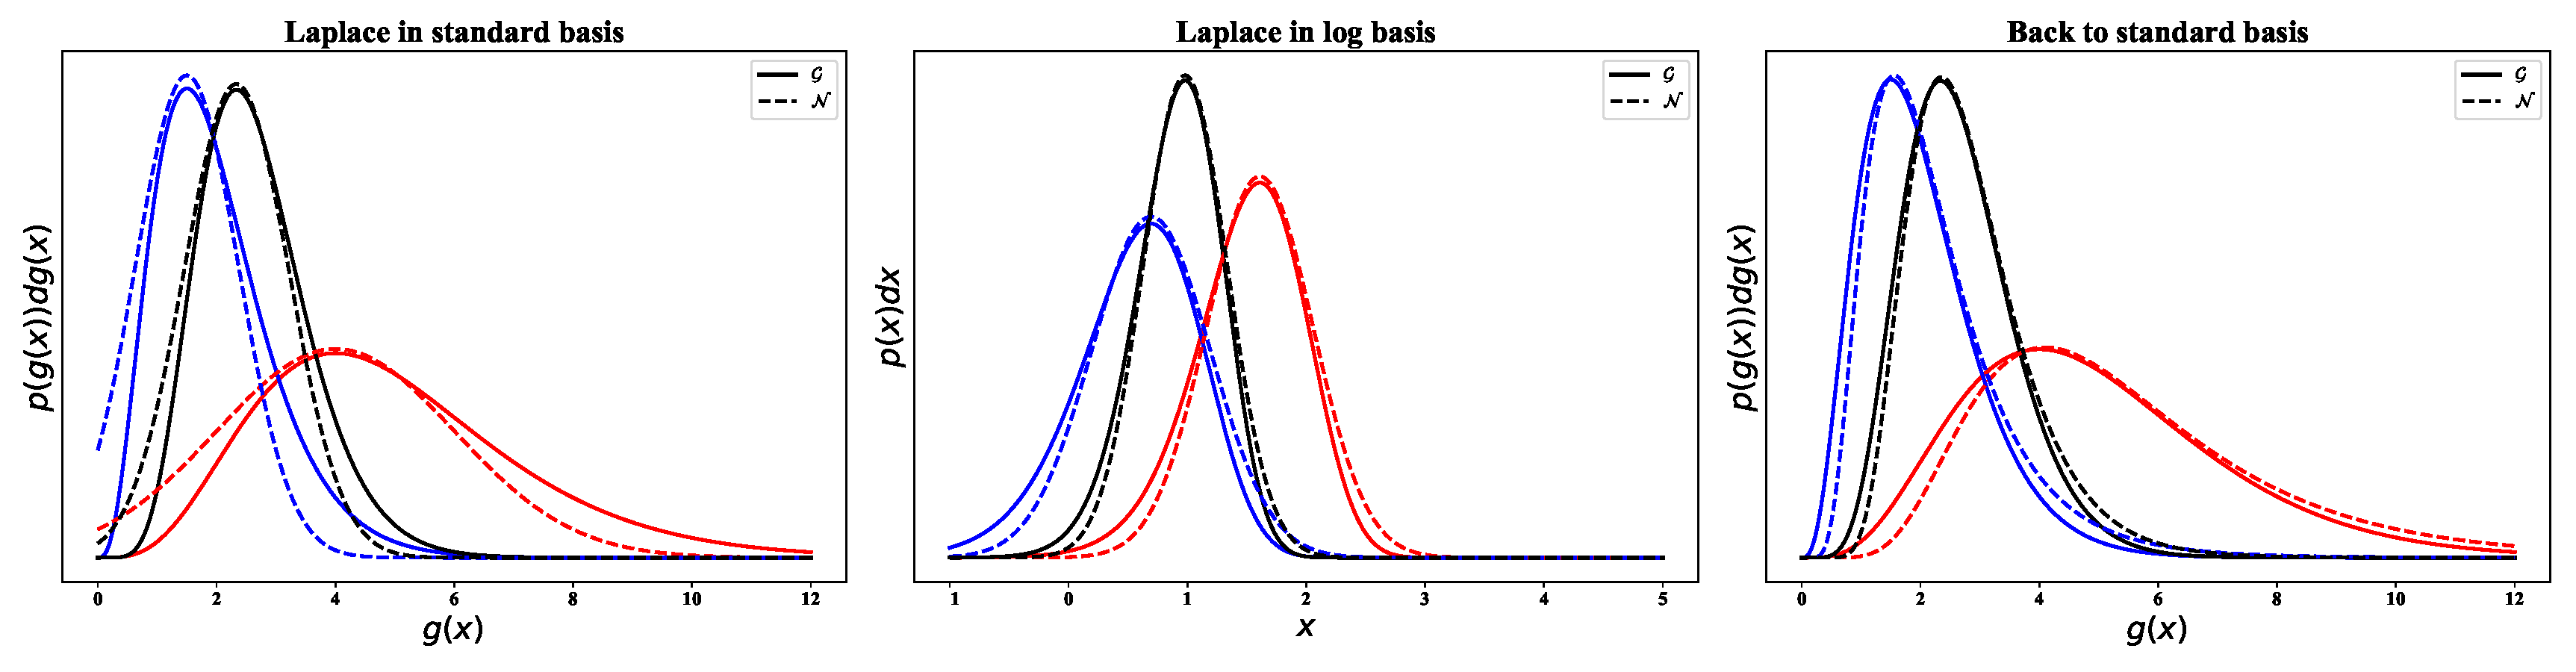
\includegraphics[width=\textwidth]{figures/Gamma_log_bridge.pdf}
	\caption{log-Bridge for Gamma distribution}
	\label{fig:gamma_log_bridge}
\end{figure}

\subsection{Sqrt-Transform of the Gamma Distribution}

\subsubsection{Sqrt-Transformation}

We transform the Gamma Distribution with the sqrt-transformation, i.e. $Y = \sqrt{X}, g(x) = \sqrt{x},x_1(y) =  g_1^{-1}(y) = -y^2, x_2(y) = g_2^{-1}(y) = y^2$ and $\left\vert\frac{\partial x_i(y)}{\partial y} \right\vert = \left\vert\frac{\partial g_i^{-1}(y)}{\partial y} \right\vert = \vert 2y \vert$. We use the same `trick' as in Subsection \ref{subsec:chi2-normal} to split up the transformation in two parts. 

\begin{subequations}
\begin{align}
\mathcal{G}_Y(y) &=  \frac{1}{2} \cdot \mathcal{G}_X(x_1(y)) \left\vert\frac{\partial x_1(y)}{\partial y} \right\vert \mathbf{1}_\wedge(y) +  \frac{1}{2} \cdot\mathcal{G}_X(x_2(y)) \left\vert\frac{\partial x_2(y)}{\partial y} \right\vert \mathbf{1}_\wedge(y) \\
&= \frac{1}{2y^2} \exp[\alpha \log(y^2) - \lambda y^2 - A(\alpha, \lambda)] |2y| \mathbf{1}_{(-\infty, 0)}(y) + \frac{1}{2y^2} \exp[\alpha \log(y^2) - \lambda y^2 - A(\alpha, \lambda)] |2y| \mathbf{1}_{[0, \infty)}(y) \\
&= \frac{1}{\sqrt{y}}\exp[2\alpha \log(y) - \lambda y^2 - A(\alpha, \lambda)] \mathbf{1}_{(-\infty, +\infty)}(y) \\
&= \frac{1}{\sqrt{y}}\exp[2\alpha \log(y) - \lambda y^2 - A(\alpha, \lambda)]
\end{align}
\end{subequations}

which is defined on the entirety of $\mathbb{R}$ and is an exponential family with $h(y) = \frac{1}{\sqrt{y}},\, \phi(y)=(\log(y), y^2), \,w=(2\alpha, -\lambda)$ and $Z(\alpha, \lambda) = \log(\Gamma(\alpha)) - \alpha \log(\lambda)$.

\subsubsection{Laplace Approximation of the sqrt-transformed Gamma Distribution}

To get the LPA of the Gamma distribution in the transformed basis we need to calculate its mode and the second derivative of the log-pdf. To get the mode we take the first derivative and set it to zero. 

\begin{align*}
\text{log-pdf: } &(2\alpha-1) \log(y) - \lambda y^2 + \alpha \log(\lambda) - \log(\Gamma(\alpha)) \\
\text{1st derivative: }&  \frac{2\alpha-1}{y} - 2\lambda y\\
\text{mode: }& \frac{2\alpha-1}{y} - 2\lambda y = 0 \Leftrightarrow y = \sqrt{\frac{\alpha-0.5}{\lambda}}\\
\text{2nd derivative: }&  -\frac{2\alpha-1}{x^2} - 2\lambda\\
\text{insert mode: }& -\frac{2\alpha-1}{\frac{\alpha-0.5}{\lambda}} - 2\lambda = -4\lambda\\
\text{invert and times -1: }& \sigma^2 = \frac{1}{4\lambda}
\end{align*}

Therefore the LPA now is $\mathcal{N}\left(\sqrt{\frac{\alpha-0.5}{\lambda}}, \frac{1}{4\lambda} \right)$.

\subsubsection{The bridge for the sqrt-transformation}

We already know how to get $\mu$ and $\sigma$ from $\lambda$ and $\alpha$. To invert we calculate $\mu = \sqrt{\frac{\alpha-0.5}{\lambda}} \Leftrightarrow \alpha = \frac{\mu^2}{\lambda}-0.5$ and insert $\lambda=\frac{4}{\sigma^2}$. In summary we have

\begin{subequations}
\begin{align}
\mu &= \sqrt{\frac{\alpha-0.5}{\lambda}} \\
\sigma^2 &= \frac{1}{4\lambda} \\
\lambda &= \frac{4}{\sigma^2} \\
\alpha &= \frac{4\mu^2}{\sigma^2}+0.5 
\end{align}
\end{subequations}

\begin{figure}[!htb]
	\centering
	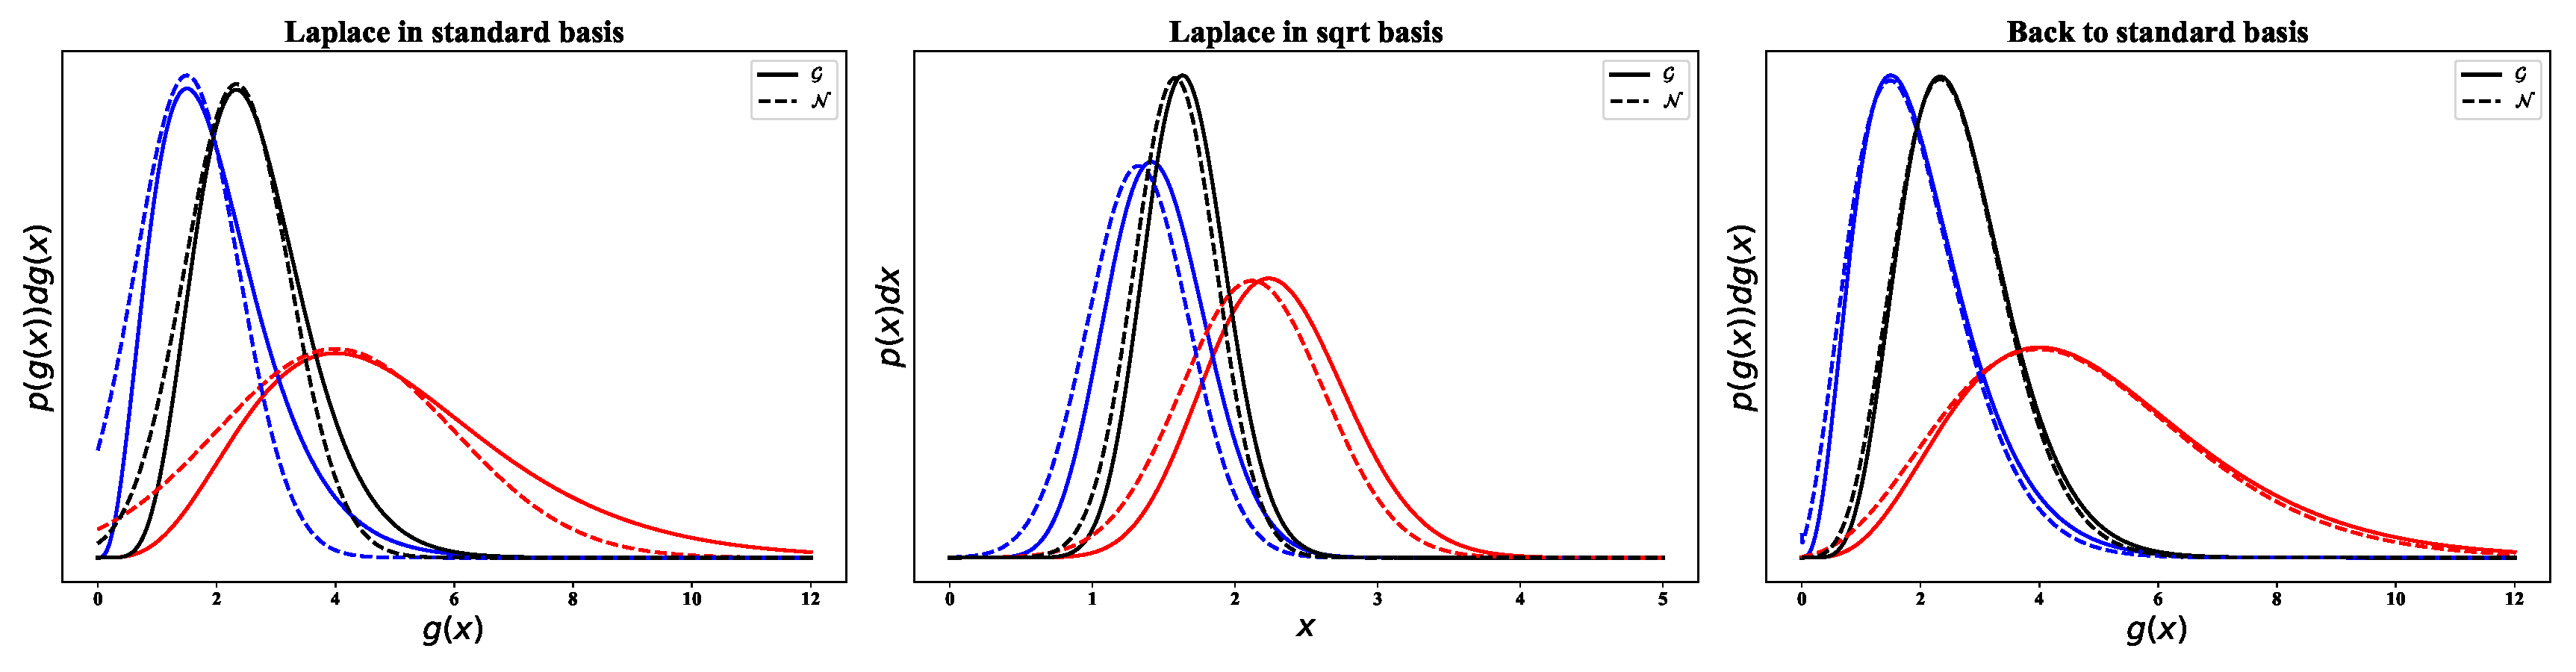
\includegraphics[width=\textwidth]{figures/Gamma_sqrt_bridge.pdf}
	\caption{sqrt-Bridge Gamma}
	\label{fig:gamma_sqrt_bridge}
\end{figure}